%\clearpage{\pagestyle{empty}\cleardoublepage}
\chapter{Rappresentazione dei dati}
\label{sec:datapresentation}
%
Una release \emph{preliminare} del sistema di monitoraggio \`e stata installata
presso un impianto fotovoltaico da 100 kWp.
%

%
In particolare, sono stati installati 1 gateway e 1 power transponder.
%
Vengono, di seguito, riportati alcuni dei grafici pi\`u significativi prodotti dal 
\emph{portale web} del sistema di monitoraggio, relativamente a questo impianto.
%
Tutti grafici presentati in questa sezione fanno riferimento allo stesso periodo 
temporale, che va dalle 06:00 alle 20:00 del 23 Giugno 2011.
%

%
In figura \ref{fig:current-power-tr} \`e riportato l'andamento della corrente immessa nella
rete di distribuzione da parte dell'impianto, per ciascuna delle tre fasi. Come \`e possibile
osservare, a meno di piccolissime variazioni, le tre curve coincidono.
%
\begin{figure}[!h]
\centering
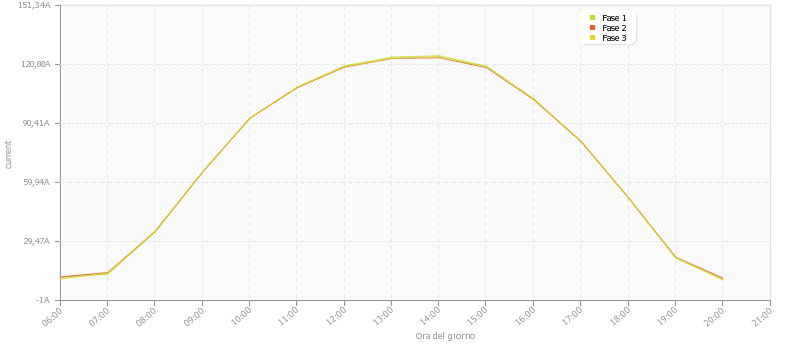
\includegraphics[width=400pt]{img/portale/current-power-transponder.png}
\caption{Corrente immessa in rete}
\label{fig:current-power-tr}
\end{figure}
%
Stesso discorso, ovviamente, vale per la tensione di rete rilevata sulle tre fasi (figura \ref{fig:voltage-power-tr}).
%

%
\begin{figure}[!h]
\centering
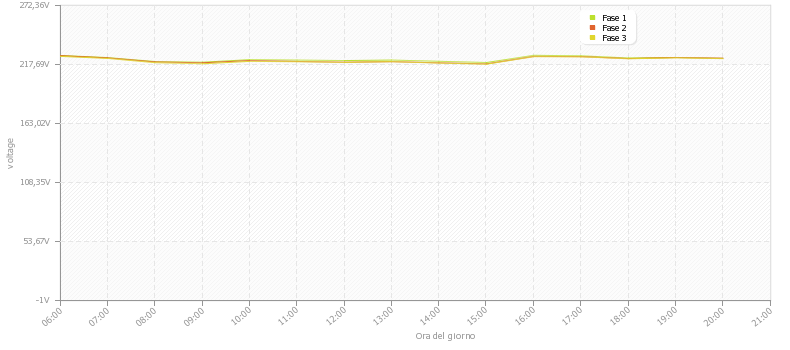
\includegraphics[width=400pt]{img/portale/voltage-power-transponder.png}
\caption{Tensione della rete di distribuzione}
\label{fig:voltage-power-tr}
\end{figure}
%

%
Le figure \ref{fig:active-power-tr} e \ref{fig:reactive-power-tr} mostrano, rispettivamente, 
la \emph{potenza attiva} e la \emph{potenza reattiva} immesse in rete.
%
Il trend della potenza attiva immessa in rete segue, come \`e ovvio che sia, l'andamento della 
corrente visto in precedenza. 
%
La somma delle tre componenti di figura \ref{fig:active-power-tr} restituisce la curva di figura 
\ref{fig:total-active-power-tr}, i.e. la potenza attiva immessa in rete da parte dell'impianto
nell'arco della giornata.
%

%
Il confronto delle curve di corrente e potenza con la curva di irraggiamento, presentata in figura 
\ref{fig:irradiance}, permette di effettuare una prima, grezza, analisi dello stato di salute 
dell'impianto; intuitivamente, infatti, tutte queste curve \emph{devono} presentare lo stesso 
andamento.
%

%
\begin{figure}[!h]
\centering
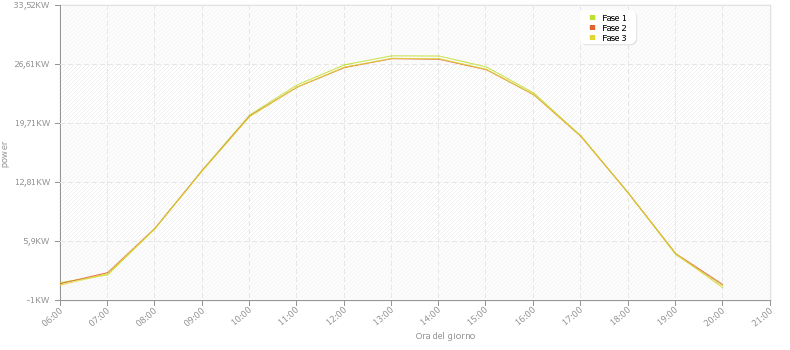
\includegraphics[width=400pt]{img/portale/active-power-transponder.png}
\caption{Potenza attiva immessa in rete}
\label{fig:active-power-tr}
\end{figure}
%

%
\begin{figure}[!h]
\centering
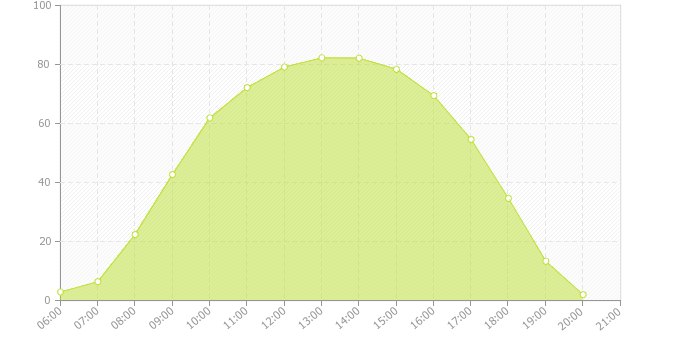
\includegraphics[width=400pt]{img/portale/potenza-giornaliera.png}
\caption{Potenza Attiva - Power Transponder}
\label{fig:total-active-power-tr}
\end{figure}
%

%
\begin{figure}[!h]
\centering
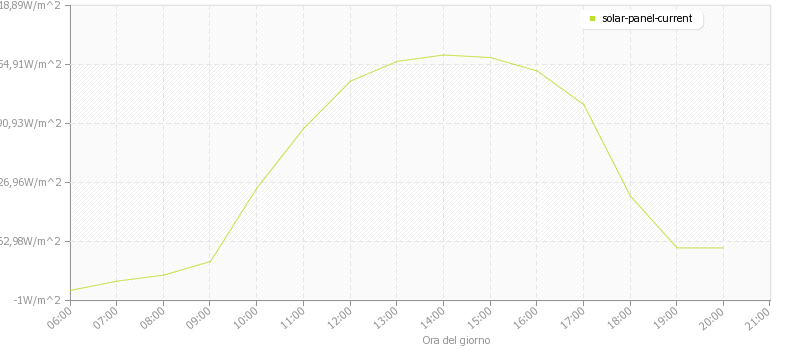
\includegraphics[width=400pt]{img/portale/radiazione-giornaliera.png} %% dire che siamo all'80% del picco
\caption{Curva di irraggiamento}
\label{fig:irradiance}
\end{figure}
%

%
La curva rappresentante il trend della potenza reattiva (figura \ref{fig:reactive-power-tr}), 
invece, permette di verificare, in impianti dotati di sistema di rifasamento, se quest'ultimo
\`e \emph{effective} oppure no. %% e nel nostro caso?
%
\begin{figure}[!h]
\centering
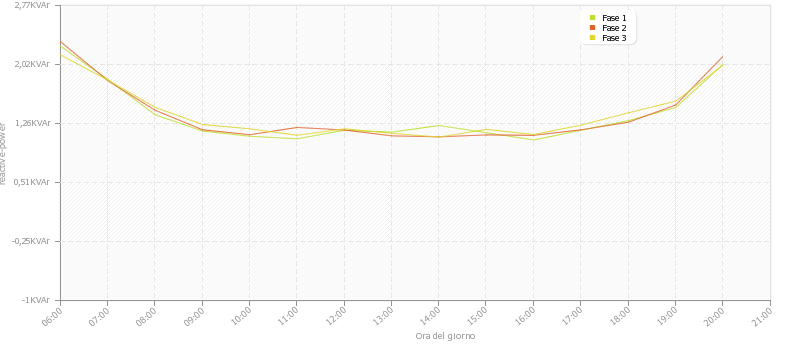
\includegraphics[width=400pt]{img/portale/reactive-power-power-transponder.png}
\caption{Potenza reattiva scambiata con la rete}
\label{fig:reactive-power-tr}
\end{figure}
%
%%Nel caso considerato, il sistema di rifasamento 
